\documentclass[a4paper, 10pt, final, garamond]{book}
\usepackage{cours-preambule}
\graphicspath{{./figures/}}

\makeatletter
\renewcommand{\@chapapp}{Contr\^ole de connaissances}
\makeatother

% \toggletrue{student}
\toggletrue{corrige}
\renewcommand{\mycol}{black}
% \renewcommand{\mycol}{gray}

\hfuzz=5.003pt

\begin{document}
\setcounter{chapter}{29}

\settype{enon}
\settype{solu}

\chapter{Solides cristallins et induction\ifstudent{~(13')}}

\begin{enumerate}[label=\sqenumi]
	\item[n]{10}
	Justifier l'existence des sites interstitiels. Donner \textbf{sans
		schéma} les positions et la population des sites T et O de la structure CFC,
	et déterminer leurs habitabilités en fonction de $r$ le rayon des sphères
	principales.
	\smallbreak
	\vspace{-5pt}
	\begin{itemize}
		\item[b]{Justification}:
		\psw{%
			Même dans les mailles compactes, il reste du vide et toutes les sphères ne
			se touchent pas~: on peut insérer de \textbf{plus petites entités}
			entre les entités principales d'une CFC.~\pt{1}
		}%
	\end{itemize}
	\smallbreak
	\vspace{-15pt}
	\begin{isd}[sidebyside align=top, interior hidden]
		\tcbsubtitle{\fatbox{\textbf{Sites tétraédriques}}}
		\begin{itemize}
			\item[bl](\tikzmark{PLA}){Position}: \psw{au centre des petits cubes
				d'arête $a/2$.}
			\item[b]{Population}: \psw{il y a 8 petits cubes et les entités
				sont dans le volume, soit $N_T = 8$.}
			\item[b]{Habitabilité}:
			\psw{%
				On a tangence \textbf{sur la moitié de la grande diagonale du petit
					cube}~: \pt{1}
				\begin{DispWithArrows*}[fleqn, mathindent=5pt]
					r + r_T \stm{=} \frac{a \sqrt{3}}{4}
					&\Lra
					\boxed{r_T = \frac{a \sqrt{3}}{4} - r}
					\Arrow{$a \stm{=} 2r \sqrt{2}$}
					\\\Lra
					\Aboxed{r_T &\stm{=} \left( \sqrt{\frac{3}{2}} - 1 \right)r \approx
						\num{0.225}r}
				\end{DispWithArrows*}
			}%
			\vspace{-15pt}
		\end{itemize}
		\tcblower
		\tcbsubtitle{\fatbox{\textbf{Sites octaédriques}}}
		\def\lspace{13}
		\begin{itemize}
			\item[bl](\tikzmark{PLR}){Position}: \psw{au centre de chaque arête et 1
				au centre.}
			\item[b]{Population}: \psw{12 arêtes et 1 centre, soit $N_O =
					1+12 \times \frac{1}{4} = 4$}
			\item[b]{Habitabilité}:
			\psw{%
				On a tangence \textbf{sur une arête}~: \pt{1}
				\begin{DispWithArrows*}[fleqn, mathindent=5pt]
					2(r + r_O) \stm{=} a
					&\Lra
					\boxed{r_O = \frac{a}{2} - r}
					\Arrow{$a = 2r \sqrt{2}$}
					\\\Lra
					\Aboxed{r_O &\stm{=} \left( \sqrt{2} - 1 \right)r \approx \num{0.414}r}
				\end{DispWithArrows*}
			}%
		\end{itemize}
	\end{isd}
	\tikz[remember picture, overlay]
	\node[left] at ([shift={(3pt,-8pt)}]pic cs:PLA) {\pt{1}};
	\tikz[remember picture, overlay]
	\node[left] at ([shift={(5pt,-6pt)}]pic cs:PLR) {\pt{1}};
	\vspace{-15pt}
	\item[n]{7}
	Soit une barre conductrice de longueur $L$ et de direction $\ux$, plongée dans
	un champ magnétique uniforme et stationnaire. On appelle $S$ sa section,
	supposée constante, et $n$ la densité d'électrons en son sein, supposée
	homogène. \textbf{Faire un schéma} d'une portion de conducteur et déterminer
	l'expression de $i$ en fonction de $e$, $n$, $S$ et $v$, puis
	\textbf{démontrer les expressions} linéique et intégrale de la force de
	\textsc{Laplace}.
	\smallbreak
	\noindent
	\begin{minipage}[c]{.65\linewidth}
		\paragraph*{Expression de l'intensité du courant}~
		\smallbreak
		\psw{%
			Les électrons passant la section pendant $\dd{t}$ sont ceux contenus dans
			le cylindre de longueur $v \dd{t}$. Dans ce cylindre, il y a $\dd{N} =
				n\times Sv \dd{t}$ électrons, soit une charge $\dd{q} = -e \dd{N} = -neSv
				\dd{t}$ \pt{1}. Ainsi,
			\[
				\boxed{\psw{i = \dv{q}{t} \stm{=} -neSv}}
			\]
		}%
	\end{minipage}
	\hfill
	\begin{minipage}[c]{.30\linewidth}
		\begin{center}
			\sswitch{
				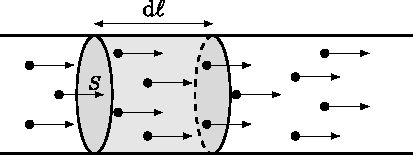
\includegraphics[width=\linewidth, draft=true]{cyl1}
			}{
				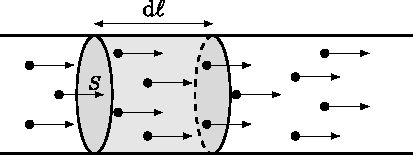
\includegraphics[width=\linewidth]{cyl1}
			}
			\vspace{-15pt}
			\captionof{figure}{Schéma fil.\protect\pt{1}}
			\label{fig:cyl1}
		\end{center}
	\end{minipage}
	\begin{isd}[sidebyside align=top]
		\paragraph*{Force subie par une section de fil}~
		\smallbreak
		\psw{%
			Dans un petit volume de longueur $\dd{\ell}$ de ce fil, il y a $\dd{N} = n
				\times S \dd{\ell}$ électrons, et chacun subit la force de
			\textsc{Lorentz} \pt{1}~; par somme~:
			alors
			\begin{align*}
				\dd{\vv{F_{\textsc{Laplace}}}}         & = -neS \dd{\ell}\vv{v}\wedge \vv{B}
				\\\Lra
				\dd{\vv{F_{\textsc{Laplace}}}}         & = -neSv (\dd{\ell}\ux)\wedge \vv{B}
				\\\Lra
				\Aboxed{\dd{\vv{F_{\textsc{Laplace}}}} & \stm{=} i \vv{\dd{\ell}}\wedge \vv{B}}
				\qed
			\end{align*}
		}%
		\vspace{-15pt}
		\tcblower
		\paragraph*{Force subie par tout le fil}~
		\smallbreak
		\psw{%
			Pour un conducteur rectiligne de A à C, on intègre~:
			\begin{align*}
				\vv{F_{\textsc{Laplace}}}
				 & \stm{=} \int_{\rm A}^{\rm B} i \vv{\dd{\ell}}\wedge \vv{B}
				\\\Lra
				\vv{F_{\textsc{Laplace}}}
				 & = i \left( \int_{\rm A}^{\rm C} \vv{\dd{\ell}}\right)\wedge \vv{B}
				\\\Lra
				\vv{F_{\textsc{Laplace}}}
				 & \stm{=} i \vv{L}\wedge \vv{B}
				\qed
			\end{align*}
		}%
		\vspace{-15pt}
	\end{isd}
	\item[n]{3} À l'aide d'un schéma, expliquer l'expérience des rails de
	\textsc{Laplace} et indiquer le sens de la force subie par le barreau.
	\smallbreak
	\begin{isd}
		\psw{%
			On réalise un circuit électrique fermé par un barreau mobile de longueur
			$\mathrm{AC} = L$. En plongeant le barreau dans un champ magnétique
			uniforme et stationnaire, le barreau subit la force de \textsc{Laplace},
			de direction indiquée ci-contre, et se met en mouvement. \pt{1}
		}%
		\tcblower
		\begin{center}
			\sswitch{
				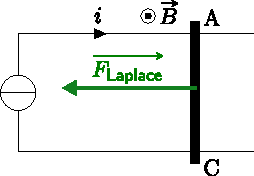
\includegraphics[height=3cm, draft=true]{rlp_2}
			}{
				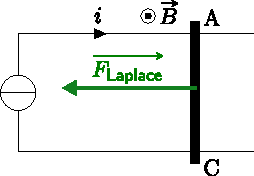
\includegraphics[height=3cm]{rlp_2}
			}
			\vspace{-15pt}
			\captionof{figure}{Schéma rails.\protect\pt{1}\psw{+}\protect\pt{1}}
			\label{fig:rlp2}
		\end{center}
	\end{isd}
\end{enumerate}
\vspace{-15pt}
\ifstudent{
	\begin{tikzpicture}[remember picture, overlay]
		\node[anchor=north west, align=left]
		at ([shift={(1.4cm,0)}]current page.north west)
		{\\[5pt]\Large\bfseries Nom~:\\[10pt]\Large\bfseries Prénom~:};
		\node[anchor=north east, align=right]
		at ([shift={(-1.5cm,-17pt)}]current page.north east)
		{\Large\bfseries Note~:\hspace{1cm}/20};
	\end{tikzpicture}
}
\end{document}
